\selectlanguage{english}
\renewcommand{\gameplayimage}{assets/first-room-en.png}
\cover{Player's manual}{Pictures without the wait. An adventure with speech.}{MSX-DOS + OPL4 / v2.0}

\thispagestyle{empty}
\begin{center}\vspace*{8mm}{\fontsize{29}{33}\selectfont\bfseries\color{accent} Return to La Mancha}\par\vspace{8mm}
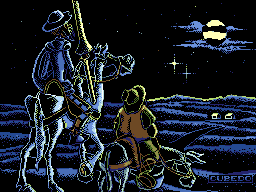
\includegraphics[width=0.85\linewidth]{assets/cover-msx2.png}
\end{center}
\textbf{Don Quijote}, published by Dinamic in 1987, brings an adventure freely inspired by Cervantes to the computer. In this illustrated text adventure, Alonso Quijano pursues his ideal of chivalry along the roads, inns and villages of La Mancha.

This MSX-DOS edition preserves the existing adventure and text. Choose the original artwork in the MSX1 version, or improved illustrations and a recoloured opening in the MSX2 version. Its additions are \textbf{fast picture loading} and \textbf{OPL4 narration} for descriptions and responses. Both parts are linked in a single session.

First you must prepare to become a knight. Further adventures then await on your journey towards Dulcinea. Look around, read carefully, and let the places and their inhabitants guide you.

\noteBox{Two editions}{Run \cmd{QUIXOTE} for English text, commands and British narration, or \cmd{QUIJOTE} for Spanish. The main examples in this manual use the English edition.}
\vfill
{\small MSX-DOS + OPL4 edition by DiHalt Studio, 2026. An unofficial adaptation and homage to the work of the original authors.}
\clearpage
\tableofcontents
\vfill
\noteBox{If Nextor is already running}{Copy all the files from \cmd{SD/} into the game folder. Select its drive, enter that folder with \cmd{CD}, then type \cmd{QUIXOTE}. The Nextor/DOS2 installation section explains the procedure.}

Before the introduction, the program shows compatible mapper RAM and detected OPL4 sample RAM. If the requirements are met, press \key{ENTER} to continue. If memory is insufficient or no compatible interface is found, it explains the reason and returns to DOS.

\sectionpage{Choose English or Spanish}
Choose the language with its launcher: \cmd{QUIXOTE.BAT} opens the English menu and \cmd{QUIJOTE.BAT} the Spanish menu. Then select MSX1 or MSX2. All versions contain both parts and support DOS1 and DOS2/Nextor.

\begin{tabularx}{\linewidth}{@{}lXX@{}}\toprule
 & English & Español\\\midrule
Distribution folder & \cmd{SD/} & \cmd{SD/}\\
Launch command & \cmd{QUIXOTE} & \cmd{QUIJOTE}\\
Game files & All; one shared package & All; one shared package\\
Narration & British English & Spanish from Spain\\\bottomrule
\end{tabularx}

Copy all files from \cmd{SD/} into one folder (the drive root under DOS1). The package contains both languages and both versions, sharing the voices and introduction. Type \cmd{QUIXOTE} or \cmd{QUIJOTE} to open its menu.

\begin{tabularx}{\linewidth}{@{}XX@{}}\toprule
English commands & Spanish commands\\\midrule
\cmd{LOOK}, \cmd{INVENTORY} & \cmd{MIRAR}, \cmd{INVENTARIO}\\
\cmd{NORTH}, \cmd{SOUTH}, \cmd{EAST}, \cmd{WEST} & \cmd{NORTE}, \cmd{SUR}, \cmd{ESTE}, \cmd{OESTE}\\
\cmd{UP}, \cmd{DOWN} & \cmd{SUBIR}, \cmd{BAJAR}\\
\cmd{READ BOOK} & \cmd{LEER LIBRO}\\
\cmd{EXAMINE WALL} & \cmd{EXAMINAR PARED}\\
\cmd{TAKE SWORD} & \cmd{COGER ESPADA}\\
\cmd{OPEN DOOR} & \cmd{ABRIR PUERTA}\\
\cmd{QUIT} & \cmd{ACABAR}\\
\cmd{SAVE}, \cmd{LOAD} & \cmd{GRABAR}, \cmd{CARGAR}\\\bottomrule
\end{tabularx}

In English, \cmd{N/S/E/W/U/D}, \cmd{L} and \cmd{I} also work. Use full command and object words, or a supported abbreviation. The names in each description will guide you.

The password announced at the end of part one is translated with the game. The start-up screen accepts either version, ignoring case and spaces. Leaving it empty and pressing \key{ENTER} always starts part one.


\sectionpage{Choose MSX1 or MSX2}
After typing \cmd{QUIXOTE} or \cmd{QUIJOTE}, the version menu appears. Type the number and press \key{ENTER}.

\begin{tabularx}{\linewidth}{@{}lX@{}}\toprule
Option & What you get\\\midrule
\cmd{1} --- MSX1 & Original pictures. Runs on MSX1 or later.\\
\cmd{2} --- MSX2 & Improved illustrations and a recoloured opening that preserves its shapes. Requires MSX2 or later.\\
\cmd{0} & Exit to DOS.\\\bottomrule
\end{tabularx}

Both options keep the same adventure, commands, speech and link between the two parts. On MSX2 or later you can choose either. If you select option 2 on MSX1, the menu explains the requirement and lets you choose again.

\begin{center}
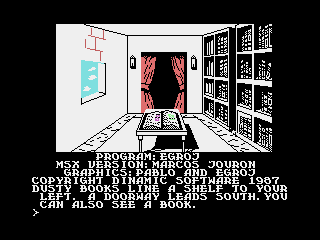
\includegraphics[width=.47\linewidth]{assets/first-room-en.png}\hfill
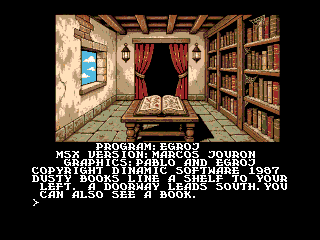
\includegraphics[width=.47\linewidth]{assets/first-room-msx2-en.png}\par
{\small The same location on MSX1 (left) and MSX2 (right).}
\end{center}

\noteBox{Upgrading an older installation}{Remove old \cmd{QUIJOTE.COM} and \cmd{QUIXOTE.COM} files before copying the new package. DOS searches for COM files before BAT files, so old executables would bypass the menu. Keep the four new game programs: \cmd{Q1ES.COM}, \cmd{Q1EN.COM}, \cmd{Q2ES.COM} and \cmd{Q2EN.COM}.}

If using a file manager, return to the DOS prompt and type \cmd{QUIXOTE} or \cmd{QUIJOTE}, or explicitly run the BAT file for your language.

\sectionpage{What you need}
\begin{tabularx}{\linewidth}{@{}>{\bfseries}p{32mm}X@{}}\toprule
Equipment & Requirement\\\midrule
Computer & MSX1 or later for option 1; MSX2 or later for option 2. An MSX keyboard.\\
Storage & MegaFlashROM SCC+ SD or a compatible MSX-DOS equivalent. Requires \textbf{512 KiB of mapper RAM}.\\
Sound & Compatible OPL4 with \textbf{2 MiB of sample RAM}, such as a Wozblaster fitted with that capacity.\\
System & MSX-DOS 1 or MSX-DOS 2 / Nextor. The same menus and programs support both.\\
Picture & A monitor or television connected to the MSX's usual video output.\\
Files & All game files from \cmd{SD/}, kept together. Allow about \textbf{13 MiB} of free space.\\
Controls & The MSX keyboard. You do not need a joystick to enter commands.\\\bottomrule
\end{tabularx}

The MSX RAM expansion and the OPL4's memory serve different purposes. \textbf{You need both capacities listed above.} Check the memory actually fitted to your cartridges, rather than relying on the model name alone.

Switch off the computer before connecting or removing cartridges. If other devices leave too few free cartridge slots, use a slot expander suitable for your set-up.

\noteBox{Use your existing system}{Start MSX-DOS or Nextor as usual. The game runs from the files in \cmd{SD/}.}

\sectionpage{Set up the computer and choose your system}
\begin{enumerate}
\item With the MSX switched off, connect the storage interface and the OPL4 to available cartridge slots.
\item Insert the SD card containing the game files.
\item Connect your display to the MSX's usual video output and prepare the computer's and OPL4's audio output. Start at a moderate volume.
\item Switch on the display and the computer.
\item Reach the DOS command prompt. If your installation starts a file manager, return to its DOS console before following the launch instructions.
\end{enumerate}

\twochoices{game files}{Files in the root directory}{Files in a game folder}{The same game and speech data}

\textbf{Nextor/DOS2} is convenient if you want to keep the game in a folder. \textbf{DOS1} requires the files to be in the partition's root directory. The drive letter depends on your installation; the examples use \cmd{B:}.

\sectionpage{Install and start under Nextor/DOS2}
Copy \textbf{all files from \cmd{SD/}} into a folder on your card. For example, use \cmd{QUIXOTE} inside \cmd{JUEGOS}.

\begin{tabularx}{\linewidth}{@{}lX@{}}\toprule
File & Purpose for the player\\\midrule
\cmd{QUIJOTE.BAT}, \cmd{QUIXOTE.BAT} & Spanish and English menus.\\
\cmd{QMENU.COM} and the four \cmd{Q1/Q2*.COM} files & Selector and game programs. Copy them all.\\
\cmd{GAME.DAT}, \cmd{ENGAME.DAT}, \cmd{Q2ES.DAT}, \cmd{Q2EN.DAT} & Both parts in each version and language.\\
\cmd{BRAND.DAT} & DiHalt Studio introduction.\\
\cmd{INDEX.DAT}, \cmd{SCORES.DAT} and their English equivalents & Narration resources.\\
\cmd{VOICE0.PCM} through \cmd{VOICE5.PCM}; \cmd{ENVOX0.PCM} through \cmd{ENVOX4.PCM} & Both languages' speech, shared by MSX1 and MSX2.\\
\cmd{VRAM.DAT}, \cmd{VRAM.IDX}, \cmd{SC5.DAT}, \cmd{SC5.IDX} & Pictures for MSX1 and MSX2.\\\bottomrule
\end{tabularx}

At the Nextor/DOS2 prompt:
\begin{quote}\ttfamily
B:\\
CD \textbackslash JUEGOS\textbackslash QUIXOTE\\
QUIXOTE
\end{quote}

Change \cmd{B:} and the path to match your card. \textbf{Enter the game folder first}: the program looks for its data in the current directory. Keep all files together with their original names.

\noteBox{What to copy and what to run}{Copy the contents of \cmd{SD/}; open \cmd{QUIXOTE.BAT} to choose a version. Run the menu from that folder, with all game files kept together.}

You do not need to flash the adventure into the MegaFlashROM. It runs from the files on the SD card.

\sectionpage{Install and start under DOS1}
\textbf{DOS1 does not support subdirectories.} Copy all files from \cmd{SD/} to the \textbf{root} of the drive used for playing. Keep their names and retain the programs, pictures and speech for both languages together.

Start your existing DOS1 installation. Select the drive containing the game and type the menu for your language:
\begin{quote}\ttfamily
B:\\
QUIXOTE
\end{quote}
For Spanish, type \cmd{QUIJOTE}. The drive letter \cmd{B:} is an example; use the letter for your disk or card.

\begin{tabularx}{\linewidth}{@{}lX@{}}\toprule
Under DOS1 & What to do\\\midrule
Location & All files directly in the drive root.\\
Language & \cmd{QUIXOTE.BAT} for English or \cmd{QUIJOTE.BAT} for Spanish.\\
Graphics version & Option \cmd{1} for MSX1 or \cmd{2} for MSX2, followed by \key{ENTER}.\\
Data & Copy every file from \cmd{SD/}; do not mix files from different editions.\\\bottomrule
\end{tabularx}

\noteBox{The same package for both systems}{DOS1 and Nextor/DOS2 use the same game files. Their location changes: the root for DOS1, the root or a folder for Nextor/DOS2. Language and graphics selection work the same way.}

After choosing a program, confirm the memory report with \key{ENTER}. If a requirement is missing, read the message and return to DOS to review your configuration before starting the game again.

\sectionpage{From start-up to your first command}
After choosing a version and pressing \key{ENTER} to confirm the memory report, the presentation begins with the DiHalt Studio logo and an OPL4 fanfare lasting about ten seconds. After it finishes, press \key{ENTER} with an empty input to start part one, or enter the password earned on completing it to start part two. Use \key{BS} to correct typing; an incorrect password lets you try again. The opening picture follows and stays on screen until you press a key to begin the chosen part.

When you enter a location with an illustration, \textbf{the picture appears first}; the description and its narration follow. Wait for the phrase to finish, or press \key{ESC} to cancel it, before typing a command.

\screenfigure{The first location: the original game's illustration, description and input prompt.}

\begin{enumerate}
\item \textbf{Picture}: illustrates the location when artwork is available for it.
\item \textbf{Text}: describes exits, objects and the consequences of your actions.
\item \textbf{Input}: the \cmd{>} symbol shows where to type your next command.
\end{enumerate}

When you complete part one, read the message and press a key when asked. Part two loads in the same session, \textbf{without entering the password again}. Its opening picture also waits for a key before continuing. Write it down to start part two in another session; it does not restore a position within a part.

\sectionpage{Controls and commands}
\begin{tabularx}{\linewidth}{@{}p{43mm}X@{}}\toprule
Action & Key or command\\\midrule
Type a command & Letters, spaces and object names. Lowercase is accepted.\\
Submit the command & \key{RETURN / ENTER}\\
Correct typing & \key{BS / Backspace}\\
Cancel the spoken phrase & \key{ESC}; release the key before cancelling another phrase.\\
Describe the location again & \cmd{LOOK} (or \cmd{L}).\\
Check what you carry & \cmd{INVENTORY} (or \cmd{I}).\\
Move & \cmd{NORTH}, \cmd{SOUTH}, \cmd{EAST}, \cmd{WEST}, \cmd{UP}, \cmd{DOWN}, when that route exists.\\
Restart the adventure & \cmd{QUIT}. Use it when you want to start again.\\\bottomrule
\end{tabularx}

Each command accepts \textbf{31 characters, including spaces}: a single line. Once it is full, further characters are ignored. You can still use \key{BS / Backspace} to edit it or \key{RETURN / ENTER} to submit it.

The simplest instruction uses \textbf{verb + noun}. Use the game's English vocabulary:
\begin{quote}
\cmd{READ BOOK}\par
\cmd{EXAMINE WALL}\par
\cmd{TAKE SWORD}\par
\cmd{OPEN DOOR}
\end{quote}
Type commands without accents, as in these examples. These illustrate vocabulary, not a sequence you must follow. Your location, the objects you carry and earlier events determine whether an action makes sense.

\noteBox{If you type while narration is playing}{Normal command entry is handled after the narration. Wait or cancel the phrase with \key{ESC}; then type your instruction and press \key{RETURN / ENTER}.}


\sectionpage{Make progress without losing your way}
Read the whole description before acting. It often mentions the exit you need or hints at something worth examining. Use \cmd{LOOK} when you want to read or hear the location again.

\begin{itemize}
\item \textbf{Explore methodically.} Write down directions and sketch a small map of places you know.
\item \textbf{Look and read.} An object may provide useful information even before you can take it.
\item \textbf{Check your inventory.} Space and the items you keep matter; the game tells you when you carry too much.
\item \textbf{Try precise actions.} If a response is unexpected, check the verb, the object and your present location.
\item \textbf{Look after the hidalgo.} Eating and resting are part of the adventure. Pay attention to its warnings.
\item \textbf{Some things remain hidden.} Darkness and the circumstances of a scene may limit what you can observe.
\end{itemize}

\begin{center}\begin{tikzpicture}[font=\small,n/.style={draw=accent,fill=paper,rounded corners,text width=26mm,align=center,minimum height=12mm},a/.style={-Latex,thick,draw=teal}]
\node[n] (m) {Look};\node[n,right=6mm of m] (e) {Examine};\node[n,right=6mm of e] (p) {Think};\node[n,right=6mm of p] (a) {Act};
\draw[a](m)--(e);\draw[a](e)--(p);\draw[a](p)--(a);
\end{tikzpicture}\end{center}

\noteBox{About saving and loading}{This edition does not add saved games on the SD card. The original \cmd{SAVE} and \cmd{LOAD} commands keep the MSX version's cassette behaviour. Do not use them expecting a saved-game file in the game folder.}

The picture does not replace the text. Some locations have no illustration; keep reading descriptions and responses to decide what to do next.

\sectionpage{If something goes wrong}
\begin{tabularx}{\linewidth}{@{}p{47mm}X@{}}\toprule
Symptom & What to check\\\midrule
DOS cannot find \cmd{QUIXOTE} & Select the correct drive. Under DOS2/Nextor, use \cmd{CD} to enter the folder containing \cmd{QUIXOTE.BAT}.\\
Error while loading files & Check all files and their names. Under DOS1 they must be in the root; under DOS2, together in the current directory.\\
The game appears but is silent & Check the OPL4 connection, volume and audio output, and confirm that it has 2 MiB of sample RAM.\\
Letters do not appear during speech & Wait for the phrase to finish or press \key{ESC}, then type your command.\\
A command is not understood & Use English vocabulary and simple phrases. Check the object's name and examine the location again.\\
The adventure starts again & Read the last message. Some actions or situations end the attempt.\\\bottomrule
\end{tabularx}





\sectionpage{Credits and rights}
\textbf{Original game}\par
Don Quijote, Dinamic Software, 1987.\par
Program: \textbf{Jorge Blecua (Egroj)}.\par
MSX version: \textbf{Marcos Jourón Berzosa}.\par
Graphics: \textbf{Pablo and Egroj}.\par
Loading picture: \textbf{Javier Cubedo}.\par
Artistic design: \textbf{Ángel Luis González}.

\textbf{MSX-DOS + OPL4 edition}\par
\textbf{DiHalt Studio, 2026}: SD loading adaptation, linked parts, fast picture loading, the MSX2 graphics version, OPL4 narration and this manual. The original adventure is preserved; the English edition translates its text and commands.

This project is an unofficial adaptation and homage. Don Quijote, its original artwork, text and other original elements remain the property of their respective rights holders. No affiliation with Dinamic or the original authors is claimed. This edition grants no rights to the original works.

The illustrations in this manual come from the game itself: the Cubedo-signed loading picture and the first-location screenshot. MSX is a trademark of its respective holders; the logo image comes from the simple-shape logo published on Wikimedia Commons. The DiHalt Studio logo belongs to the project.

\textbf{Further reading and provenance}\par
The game entry, credits and original-manual transcription preserved by Computer Emuzone were used to check the history and names:\par
\href{https://computeremuzone.com/ficha/151/don-quijote}{computeremuzone.com/ficha/151/don-quijote}.\par
The \cmd{SOURCES.md} file beside this manual's sources records the provenance of the illustrations and information consulted.

\vfill
\textcolor{accent}{\textbf{Preserve the adventure. Share your observations.}}\par
Source code and documentation are available in the \href{https://github.com/DiHaltStudio/donquijote-msx1-opl4-en-es}{DiHalt Studio GitHub repository}. Please improve the game if you feel so!
